% Hyperbolic paraboloid z = xy: the lines x = c (blue) and y = c (red) lie on it.
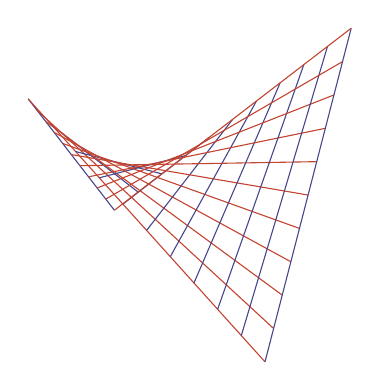
\begin{tikzpicture}[scale=1.6]
\draw[MidnightBlue!80] (-1.2817,0.6024) -- (-0.5977,-0.2812);
\draw[BrickRed!80] (-1.2817,0.6024) -- (0.5977,-1.4847);
\draw[MidnightBlue!80] (-1.0938,0.3937) -- (-0.4097,-0.1367);
\draw[BrickRed!80] (-1.2133,0.5140) -- (0.6661,-1.2199);
\draw[MidnightBlue!80] (-0.9058,0.1850) -- (-0.2218,0.0077);
\draw[BrickRed!80] (-1.1449,0.4256) -- (0.7345,-0.9550);
\draw[MidnightBlue!80] (-0.7179,-0.0238) -- (-0.0339,0.1522);
\draw[BrickRed!80] (-1.0765,0.3373) -- (0.8029,-0.6902);
\draw[MidnightBlue!80] (-0.5300,-0.2325) -- (0.1541,0.2967);
\draw[BrickRed!80] (-1.0081,0.2489) -- (0.8713,-0.4254);
\draw[MidnightBlue!80] (-0.3420,-0.4412) -- (0.3420,0.4412);
\draw[BrickRed!80] (-0.9397,0.1606) -- (0.9397,-0.1606);
\draw[MidnightBlue!80] (-0.1541,-0.6499) -- (0.5300,0.5856);
\draw[BrickRed!80] (-0.8713,0.0722) -- (1.0081,0.1043);
\draw[MidnightBlue!80] (0.0339,-0.8586) -- (0.7179,0.7301);
\draw[BrickRed!80] (-0.8029,-0.0161) -- (1.0765,0.3691);
\draw[MidnightBlue!80] (0.2218,-1.0673) -- (0.9058,0.8746);
\draw[BrickRed!80] (-0.7345,-0.1045) -- (1.1449,0.6339);
\draw[MidnightBlue!80] (0.4097,-1.2760) -- (1.0938,1.0191);
\draw[BrickRed!80] (-0.6661,-0.1929) -- (1.2133,0.8987);
\draw[MidnightBlue!80] (0.5977,-1.4847) -- (1.2817,1.1635);
\draw[BrickRed!80] (-0.5977,-0.2812) -- (1.2817,1.1635);
\end{tikzpicture}
